% MNS project 2010 slides
% 
% Luís Francisco Seoane Iglesias
% Mirko Dietrich - mirko.dietrich -AT- bccn-berlin -DOT- de
% 

\documentclass{beamer}
	\usepackage{color}

\title{Spike-timing-dependent plasticity}
\author{Lu\'{i}s Francisco Seoane Iglesias \& Mirko Dietrich}
\date{\today}

\logo{
\includegraphics[scale=0.2]{graphics/bccn_logo_berlin}}

\begin{document}

\frame{\titlepage}

\section*{Outline}
\frame{
  \tableofcontents
}

\section{Introduction}
\subsection{Overview of the Beamer Class}
\frame
{
  \frametitle{Spike-time-dependent}

  \uncover{
    Based upon \textbf{integrate-and-fire} neuron model: $\tau_{m} \frac{dV}{dt} = V_{rest} - V + \textcolor{red}{g_{ex}(t)}(E_{ex} - V) + \textcolor{blue}{g_{in}(t)}(E_{in} - V)$ \\
    \vspace{1em}
    \uncover<2->{$\textcolor{red}{g_{ex}(t)}\rightarrow g_{ex}(t) + \bar{g_a} $ \\
      $\textcolor{blue}{g_{in}(t)}$}
  }
}

\section{Demo}

	\begin{frame} 
		\begin{columns} 
			\column{0.5\textwidth} 
				\begin{figure} 
					\centering
					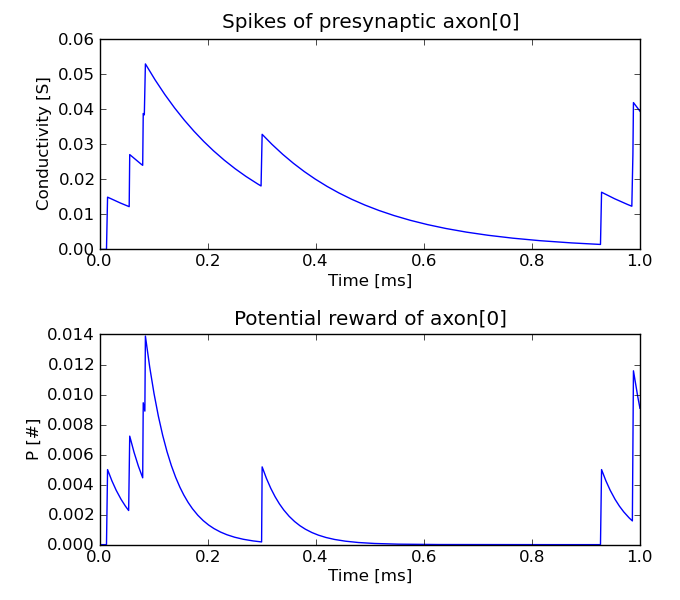
\includegraphics[width=\textwidth]{graphics/demo/fig01} 
				\end{figure} 
			\column{0.5\textwidth} 
				\begin{itemize} 
					\item Axons spike with a certain frequency. 
					\item When spike, a \alert{potential \emph{reward}} accumulates. 
				\end{itemize}
		\end{columns}
	\end{frame}
	
	\begin{frame} 
		\begin{columns} 
			\column{0.5\textwidth} 
				\begin{figure} 
					\centering
					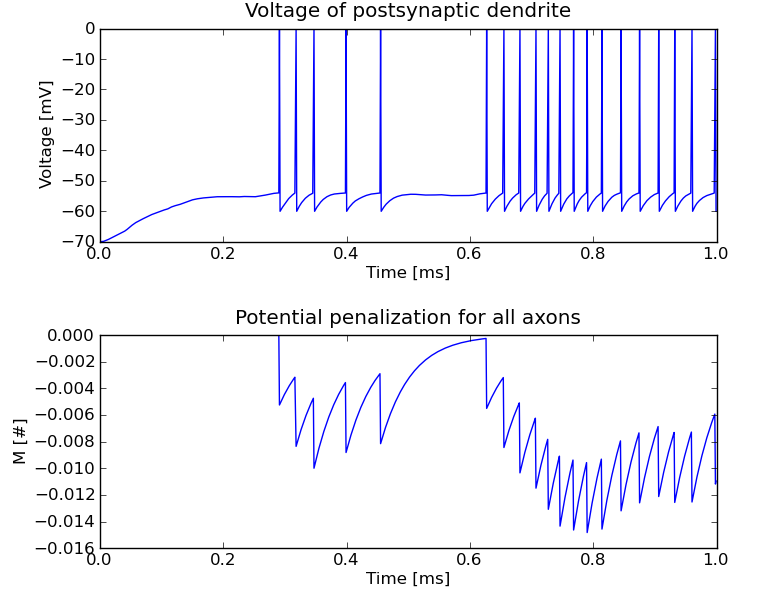
\includegraphics[width=\textwidth]{graphics/demo/fig02} 
				\end{figure} 
			\column{0.5\textwidth} 
				\begin{itemize} 
					\item The dendrite spikes induced by the axons. 
					\item A \alert{\emph{penalty} function} also accumulates, elicited by the spike of the dentrite. 
				\end{itemize}
		\end{columns}
	\end{frame}

\end{document}
 